\chapter{Requerimientos}
\section{Introducción}
Dentro del aplicativo, se plantean un serie de requerimientos de tipo cliente y tipo desarrollador,los cuales buscan plantear plasmar las necesidades del cliente y las temas que deben tener en cuenta los desarrolladores para crear un producto. Dichos requerimientos serán abordados y explicados a lo largo de este capítulo.
\section{Requerimientos tipo C}
Estos son directamente los requerimientos funcionales del cliente, son aquellos requerimientos que están completamente ligados con las necesidades que necesita el cliente.

A continuación se espeficarán y describirán cada uno de los casos de uso expuestos:


\section{Diagrama de Casos de Uso}
Estos diagramas son los que permiten mostrar la relación que existe entre los usuarios y el sistema, mediante ellos se busca explicar qué es lo que esperan que el aplicativo haga.

\section{Diagrama de Secuencia}
Este tipo de diagrama es el que permite entender cómo se espera que funcione el aplicativo ante los deseos del usuario, están muy relacionados con los diagramas de casos de uso, relacionan lo que quieren los usuarios con el funcionamiento interno del sistema para llevarlo a cabo.

\section{Diagramas de Comunicación}
Este diagrama es un diagrama es quizás el más complejo de los tres, no porque tenga una realización díficil, más bien es un diagrama que busca mostrar como es la interacción entre los distintos objetos que componen el requerimiento, está muy ligado con el diagrama de secuencia, pues muestra información muy similar.


 A continuación se muestran los diagramas de casos de uso, secuencia y comunicación respectivamente que se han encontrado para este aplicativo:

\begin{figure}[h!]
	\centering
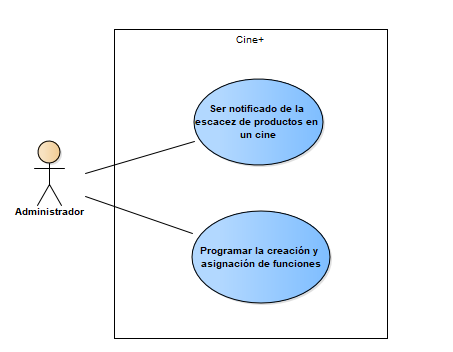
\includegraphics[width=.6\linewidth]{diseno/requerimientos/imgs/casosUso1}
	\caption{Casos de uso del sistema}
\end{figure}

\begin{figure}[h!]
	\centering
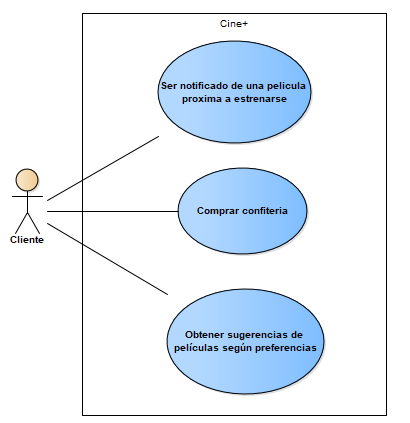
\includegraphics[width=.6\linewidth]{diseno/requerimientos/imgs/casosUso2}
	\caption{Casos de uso del sistema}
\end{figure}


\begin{figure}[h!]
\centering
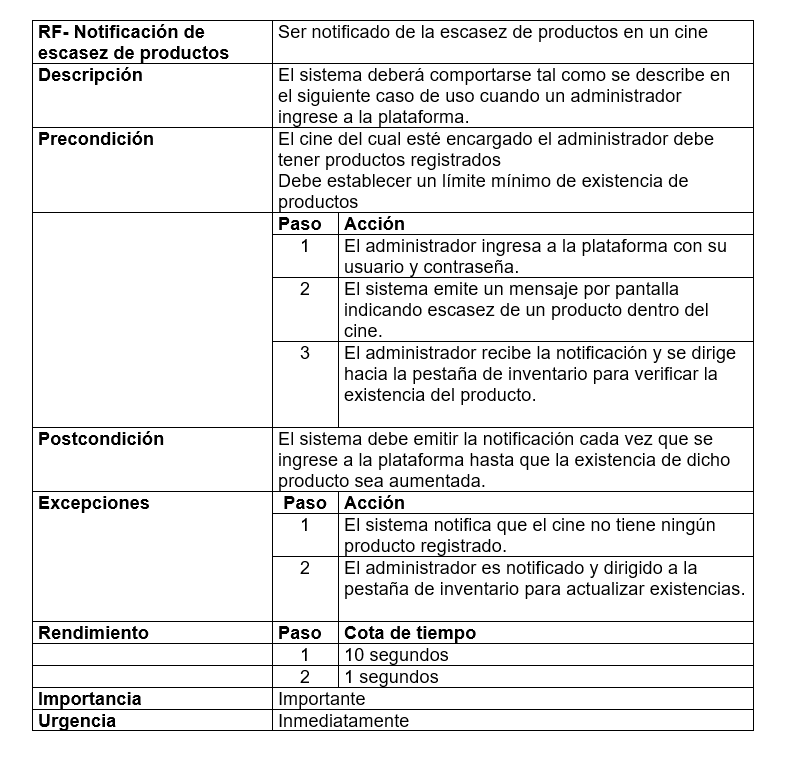
\includegraphics[width=.8\linewidth]{diseno/requerimientos/imgs/casos1}
	\caption{Requerimientos Tipo C}
\end{figure}
\newpage
\begin{figure}[h!]
\centering
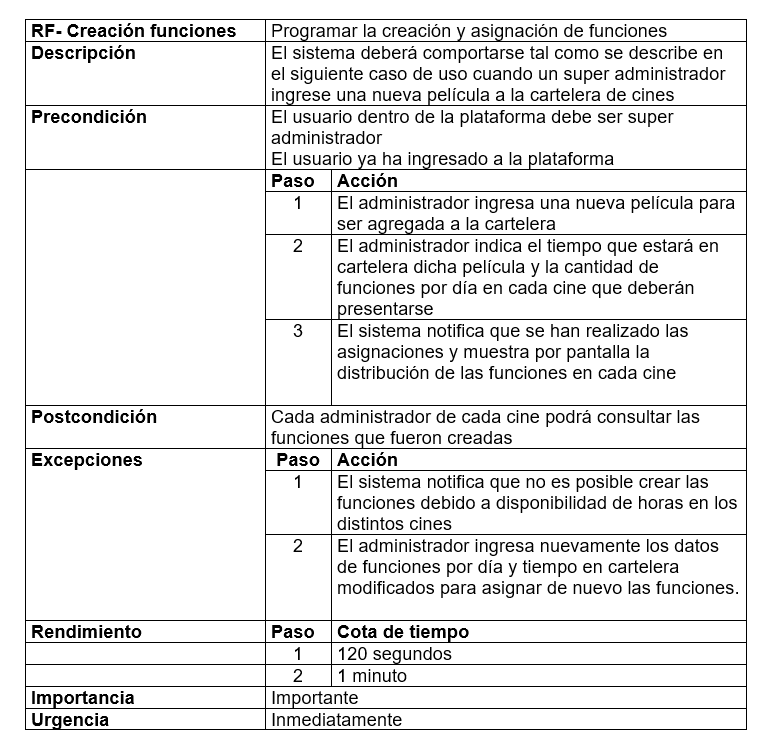
\includegraphics[width=.8\linewidth]{diseno/requerimientos/imgs/casos2}
	\caption{Requerimientos Tipo C}
\end{figure}
\newpage
\begin{figure}[h!]
\centering
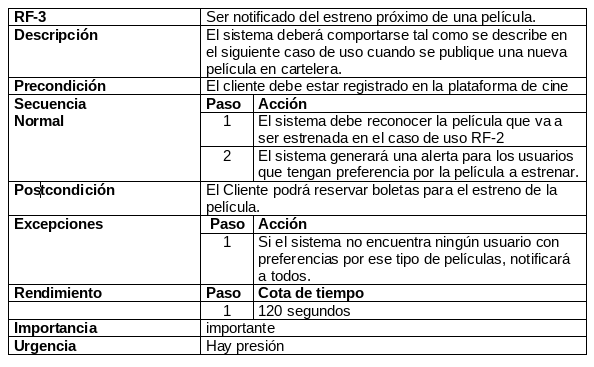
\includegraphics[width=.8\linewidth]{diseno/requerimientos/imgs/casos3}
	\caption{Requerimientos Tipo C}
\end{figure}
\newpage
\begin{figure}[h!]
\centering
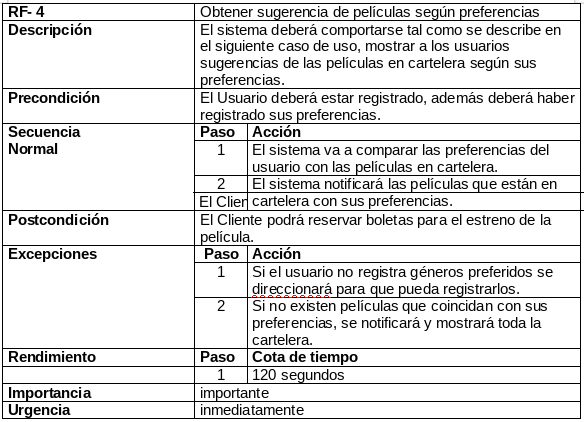
\includegraphics[width=.8\linewidth]{diseno/requerimientos/imgs/casos4}
	\caption{Requerimientos Tipo C}
\end{figure}
\newpage
\begin{figure}[h!]
\centering
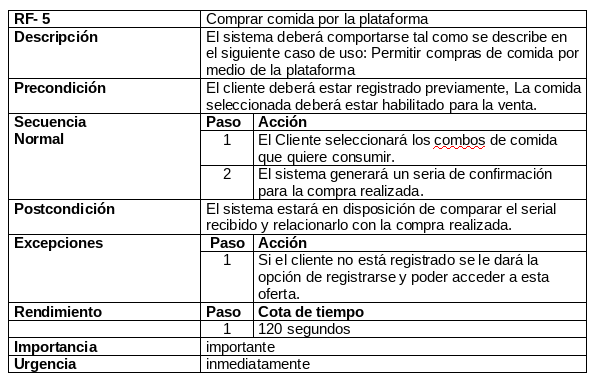
\includegraphics[width=.8\linewidth]{diseno/requerimientos/imgs/casos5}
	\caption{Requerimientos Tipo C}
\end{figure}


\begin{figure}[h!]
\centering
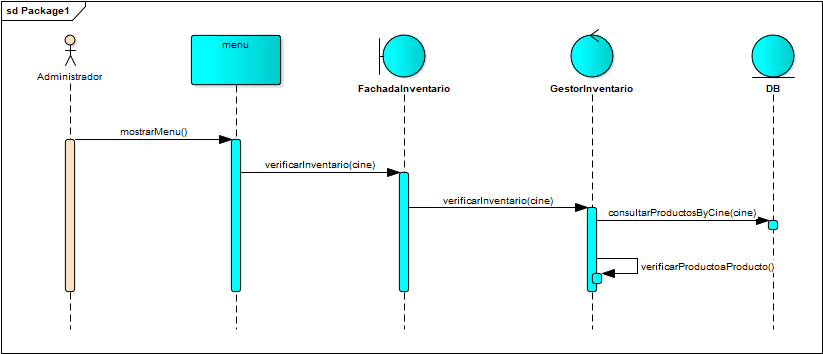
\includegraphics[width=1\linewidth]{diseno/requerimientos/imgs/EscacezSec}
	\caption{Diagrama de secuecia: Notifición de escacez de un producto}
\end{figure}
\begin{figure}[h!]
\centering
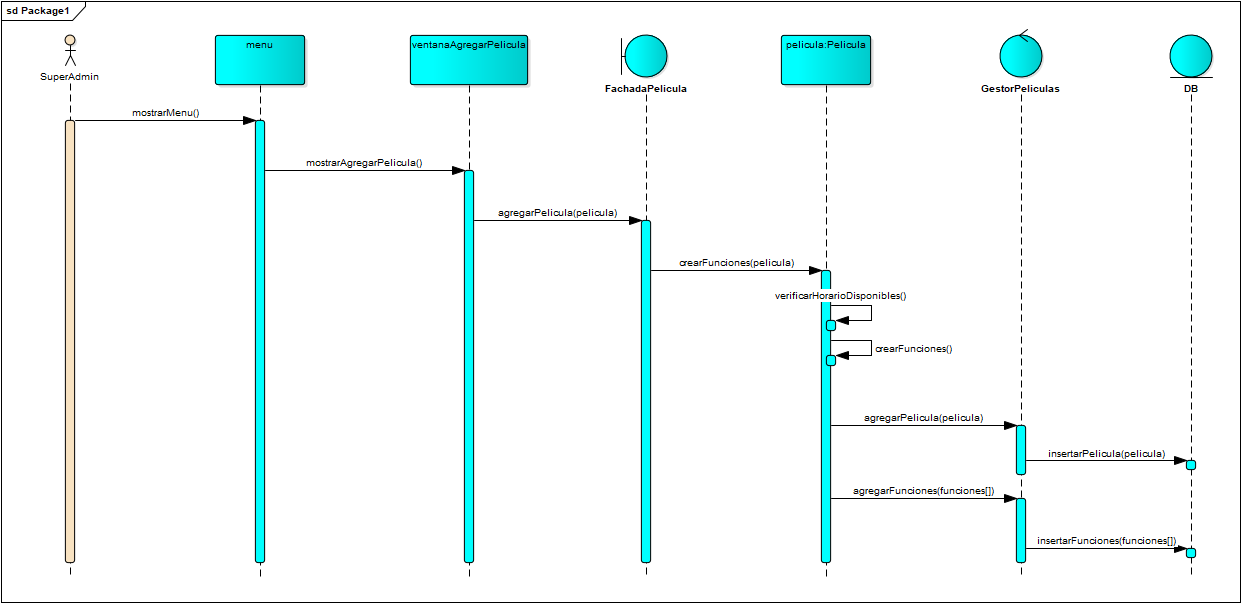
\includegraphics[width=1\linewidth]{diseno/requerimientos/imgs/FuncionesSec}
	\caption{Diagrama de secuecia: Programar la asignación y creación de funciones}
\end{figure}
\begin{figure}[h!]
\centering
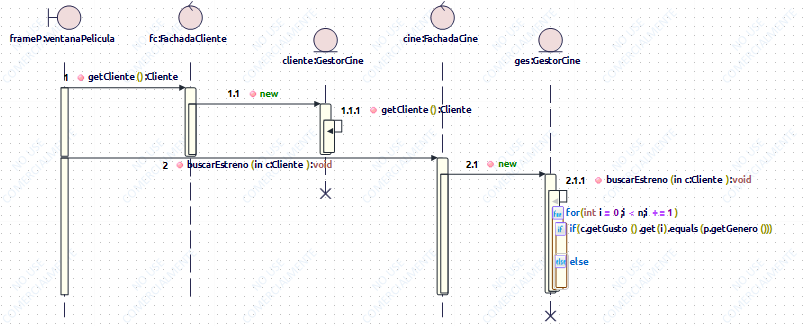
\includegraphics[width=1\linewidth]{diseno/requerimientos/imgs/EstrenosSec}
	\caption{Diagrama de secuecia: Ser notificado del estreno próximo de una película}
\end{figure}
%DIAGRAMA DE SECUENCIA DE OBTENER SUGERENCIAS <-------------------------- !
%\begin{figure}[h!]
%\centering
%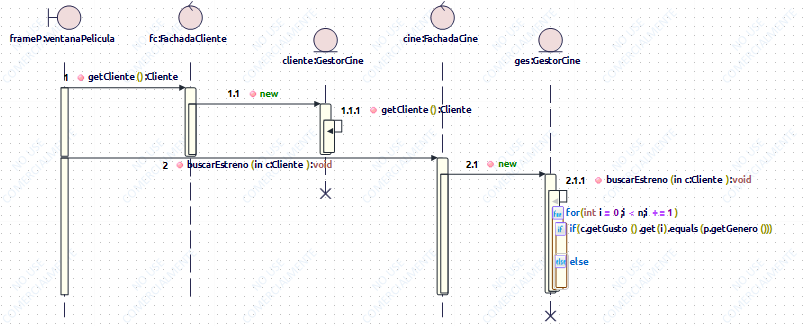
\includegraphics[width=1\linewidth]{diseno/requerimientos/imgs/EstrenosSec}
%	\caption{Diagrama de secuecia: Ser notificado del estreno próximo de una película}
%\end{figure}
\begin{figure}[h!]
\centering
\includegraphics[width=1\linewidth]{diseno/requerimientos/imgs/CompraCombosSec}
	\caption{Diagrama de secuecia: Comprar comida por la plataforma}
\end{figure}




\begin{figure}[h!]
\centering
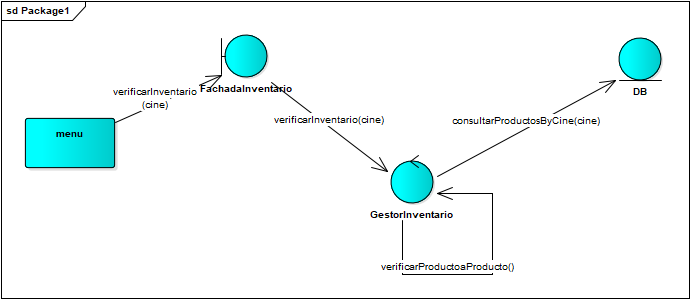
\includegraphics[width=1\linewidth]{diseno/requerimientos/imgs/EscacezCom}
	\caption{Diagrama de comunicación: Notificación de escacez de un producto}
\end{figure}


\begin{figure}[h!]
\centering
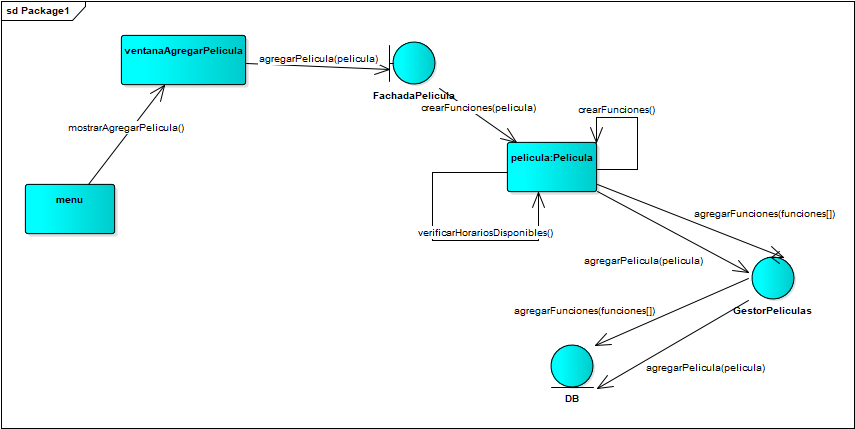
\includegraphics[width=1\linewidth]{diseno/requerimientos/imgs/FuncionesCom}
	\caption{Diagrama de comunicación: Programar creación y asignación de funciones}
\end{figure}

\begin{figure}[h!]
\centering
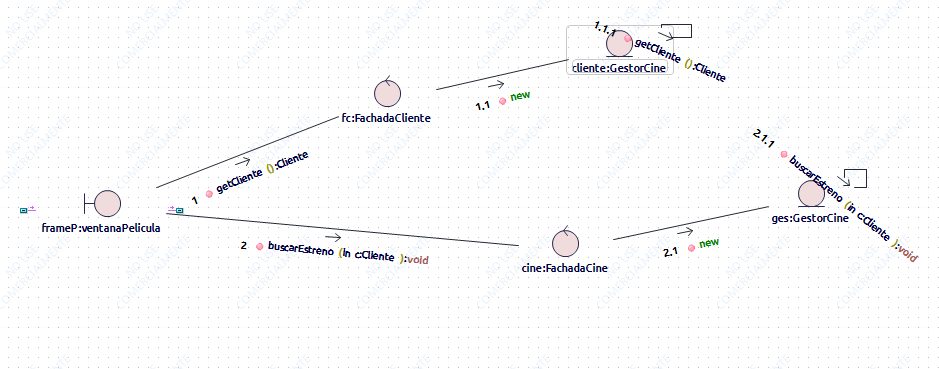
\includegraphics[width=1\linewidth]{diseno/requerimientos/imgs/EstrenoCom}
	\caption{Diagrama de comunicación: Ser notificado del estreno próximo de una película}
\end{figure}
%DIAGRAMA DE COMUNICACIÓN: SUGERENCIAS DE PELICULAS <----------- !
%\begin{figure}[h!]
%\centering
%\includegraphics[width=1\linewidth]{diseno/requerimientos/imgs/CompraCombosSec}
%	\caption{Diagrama de secuecia: Comprar comida por la plataforma}
%\end{figure}
\begin{figure}[h!]
\centering
\includegraphics[width=1\linewidth]{diseno/requerimientos/imgs/CompraCombosCom}
	\caption{Diagrama de comunicación: Comprar comida por la plataforma}
\end{figure}
